% need for program correctness

Since the beginning of programming languages, the problem of program correctness has been an issue. 
Especially, this is the case today when complex software applications  enter into our daily life and perform actions 
which may potentially compromise confidential data (credit cards) or the performance of the
 computer system they are executed on (e.g. installing software which may format the hard disk of our PC).
Also, errors in software conception may have disastrous effects, for instance
the crash of the European Ariane 5 launcher due to an under testing. More over, software correctness
 plays a crucial role in the overall software quality  in cases the latter take part in the automatic 
control of engines which may put in danger lives, like airplanes or subways.


% source verification. Helps developers, software audit 
Thus, a necessary phase in the program development is the validation of the program implementation, during which 
the producer checks if the written code conforms to her/his intentions. 


A widely used approach is program testing. However, this technique is not capable
to cover all the cases of the input space and thus, although the tests have been successful, 
the implementation may still contain errors. This, of course, is not desirable in particular in the case of critical 
program applications as is the case for applications which target the domains mentioned above.

 Another possibility is to use formal verification methods. 
Contrary to program testing,  program verification guarantees that if the verification procedure  
has been successful then the implementation respects the initial requirements for the software. There are few approaches 
in formal verification as for instance model checking and program logic. In this thesis, we will focus on the second approach.  
In Fig. \ref{intro:srcVerif}, we give a general outline of the architecture for verifying source code programs.
\begin{figure}[ht!]
%\begin{frameit}
\begin{center}
%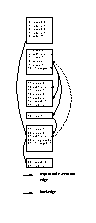
\includegraphics{bc.eps}
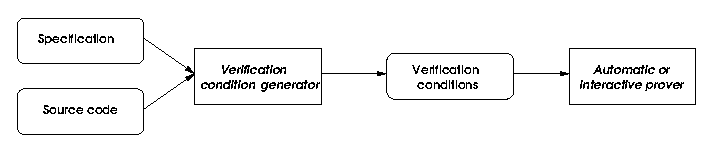
\epsfig{file=figs/sourceVerification.eps}%, height=5in,  width=1.5in}
\caption{\sc Source verification}
\label{intro:srcVerif}
\end{center}
%\end{frameit}
\end{figure}

As we can see from the figure, the architecture relies on the following components:
\begin{itemize} 
   \item specification of the implementation which expresses the intended behavior of the source program. The annotations
         are written in a formal specification language. 
   \item an algorithm which  generates logical (verification) conditions  from the annotations and the program.
         Such an algorithm is usually called verification condition generator. 
         The generated verification conditions are such that their truthfulness guarantees that the implementation respects the program specification  and thus,
	 that the implementation respects its intended behavior.
    
   \item a system for showing the validity of the verification conditions. This is normally done either by an automatic decision 
         procedure or interactive theorem prover.
         Automatic decision procedures do not need user interaction.
         However, automation cannot deal with difficult theorems because of the undecidability of the logic.
	 Interactive prove assistant is an alternative which is 
	 more powerful and can more often ``say'' if something holds or not. Of course, because of the undecidability 
	 even  interactive prove assistants may fail to decide if a proposition holds or not. Although interactive prove assistants
	 systems are more reliable they need a user expertise in theorem proving and logic. 
	 Thus, depending on the complexity of the verification conditions, an automatic decision procedure or an interactive system is used.

   \end{itemize} 



 The field of formal  verification is well studied and several  tools exist for
dealing with  source verification using program logic. We should mention in the list of the verification tools tailored to source languages
the Caveat\footnote{http://www-list.cea.fr/labos/fr/LSL/caveat/index.html} verification framework  for C,
 Caduceus\footnote{http://why.lri.fr/caduceus/index.fr.html} for C,  the extended static checker
esc/java \cite{escjava}, the Loop tool \cite{jacobs03java},
Krakatoa \cite{marche03krakatoa}, Jack \cite{BRL-JACK}, etc. These tools are tailored to a source language and thus,
 are helpful for the development process. For instance, the developer may use such verification tools for discovering program bugs and
 errors. More generally, verification on source code allows the code producer to audit the quality of a software implementation.
 
%source verification not always appropriate
Although  program logics  guarantees source program correctness, it does not say anything about the executable code
resulting from the source compilation. Thus, source verification requires a  trust in the compiler.
However,  such a compromise is not always admissible. 
% mobile code



This is in particular  the case for mobile code scenarios  where a code client
executes an unknown or untrusted application. 
Fig. \ref{intro:mobile} shows a schemata of mobile code scenarios. From the figure, we can see that in such scenarios 
there are two counter parts:  a code producer and a code client. The producer generates the code and the client 
receives the generated code. However, the client  normally does not have any evidence that the code respects the 
his requirements.
\begin{figure}[ht!]
%\begin{frameit}
\begin{center}
%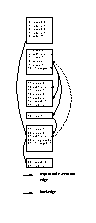
\includegraphics{bc.eps}
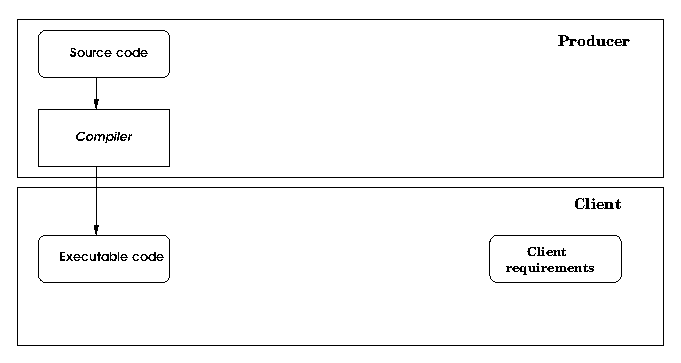
\epsfig{file=figs/mobileCode.eps}
\caption{\sc Mobile code}
\label{intro:mobile}
\end{center}
%\end{frameit}
\end{figure} 

Examples for a mobile code scenario can be the downloading of software components  via internet  and their execution  on a user system which can be a personal computer,
 PDAs, embedded systems, etc. These software components could be from user specific applications to patches for the operating system.

 


%Bytecode verification
Thus, it is more suitable to perform the verification  directly on the executable or interpreted code.
First, because the executable is normally not accompanied by the corresponding source code and second, even if it were this would require 
trust in the compiler. In particular, this means that the client should perform \textit{ verification over the executable code}. This would mean that  the client should 
have the infrastructure shown above in Fig. \ref{intro:srcVerif}.but this time for the executable or interpreted code.

\begin{figure}[ht!]
%\begin{frameit}
\begin{center}
%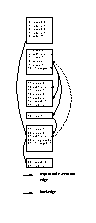
\includegraphics{bc.eps}
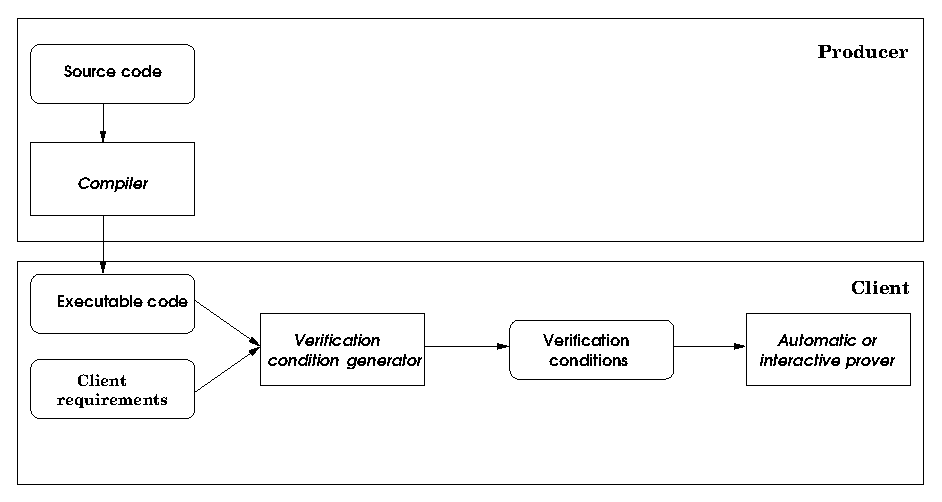
\epsfig{file=figs/mobileCodeVerif.eps}
\caption{\sc Mobile code verification}
\label{intro:mobileVerif}
\end{center}
%\end{frameit}
\end{figure}

Providing mechanisms for verification over the executable or interpreted code gives the client the possibility to check if the application respects the requirements of the client system.
However, the process of theorem proving is an expensive computational procedure and  the client system may potentially not be willing to 
slow down its execution for verifying the unknown code.
Especially, this is the case for small devices which rely on limited computational resources. 

%PCC
 The Proof Carrying Code paradigm (PCC) and the certifying compiler proposed by G.Necula \cite{DesNecLee98} gives a solution to this problem. In the traditional PCC architecture, untrusted code is accompanied by a proof which certifies that the code is in compliance with the client  requirements. In Fig. \ref{intro:PCC}, we show  the basic components of such framework and the relation between them. The code producer uses the so called certifying compiler. The certifying compiler consists of a compiler from source code
to executable (or interpreted bytecode) which generates also annotations for the executable code  and a certifier. The certifier assembles the verification condition generator
over the executable and an automatic decision procedure which will generate the proof for the verification condition generator. The producer sends the 
executable code with annotations  and the proof to the client.
The client then does not have to prove the program. Rather, he generates the verification conditions over the received code  and his requirements and
then checks if  the proof accompanying the code is a proof for the generated verification conditions. Checking a proof w.r.t. a logical statement is much easier then finding  
its proof.  For this, type checking algorithms are used as  the verification conditions are interpreted as types and the proofs are interpreted as expressions. 
The complexity of type checking algorithms is small and thus, do not compromise  the performance of the client system.
\begin{figure}[ht!]
%\begin{frameit}
\begin{center}
%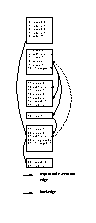
\includegraphics{bc.eps}
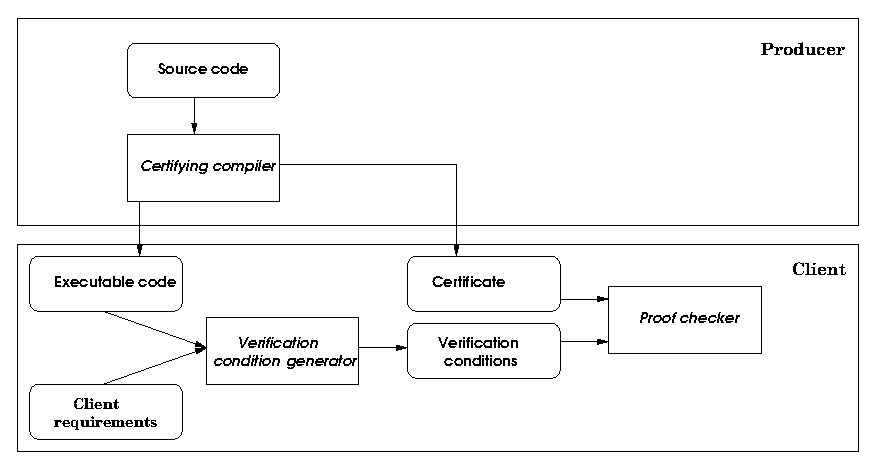
\epsfig{file=figs/PCC.eps}
\caption{\sc Proof carrying code architecture for mobile code}
\label{intro:PCC}
\end{center}
%\end{frameit}
\end{figure}



% generate the certificate over the source code
However, because traditional PCC is completely automatized, it can only deal with safety properties, like well typedness or safe memory read and write access.
These properties are very important as they guarantee that the execution of the whole system will not be violated by the untrusted application.
However, restricting the verification mechanism only to safety properties is not satisfactory, because there are 
potentially scenarios where the client security policy may involve more complex properties over the untrusted application.
For instance, the client may have functional requirements over the unknown code. An example is  when an updated version  of an interface   implementation
 is downloaded on the  client computer system and patches an old implementation of the interface. In this cases, the client system needs guarantees
 that the unknown software component respects the interface specification.
In such situations, traditional PCC is not appropriate as it will fail to generate the proof automatically. 


A solution to this problem is to give up automation in the certificate generation and thus, make the process of  the proof generation 
on the producer site interactive as shown in Fig. \ref{intro:PPO}. As you can see in the figure, we propose that  the producer site
 \textit{generates the certificate interactively over the source code}. The advantage of 
such an approach  is that the interactive proof will allow to identify bugs in the source code and
 correct them until the source becomes conform with the client  requirements. 
Moreover,  interactive verification over source code allows to identify  points in the source program which 
must be enforced with  annotations (typically, loop invariants)
 that will allow the verification conditions to get provable. 
However, there are several points which need to be clarified.
The first one is how the client may use a source code certificates for the verification of its executable counterpart.
This is actually possible as verification conditions over source and low level code are equivalent if the low level 
code has been produced by a non optimizing compiler. However, this equivalence is not sufficient to make things work.
In particular, sending the executable code and its certificate is not sufficient for the client to check correctly the program.
 As we said above, the generation of the certificate on the producer site, requires potentially enforcement of
 the program with annotations. 
 Remind that the validation of the executable program on the client side  involves the generation of the verification
 conditions again. If the client does not have the annotation enforcement for the program, he will not succeed to type
check the verification conditions that he generated against the received certificate, even if the program is correct. 
For this, we propose a compiler from source annotations to annotations on the level of the executable (interpreted) code.



 

    \begin{figure}[ht!]
%\begin{frameit}
\begin{center}
%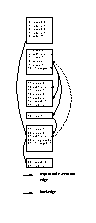
\includegraphics{bc.eps}
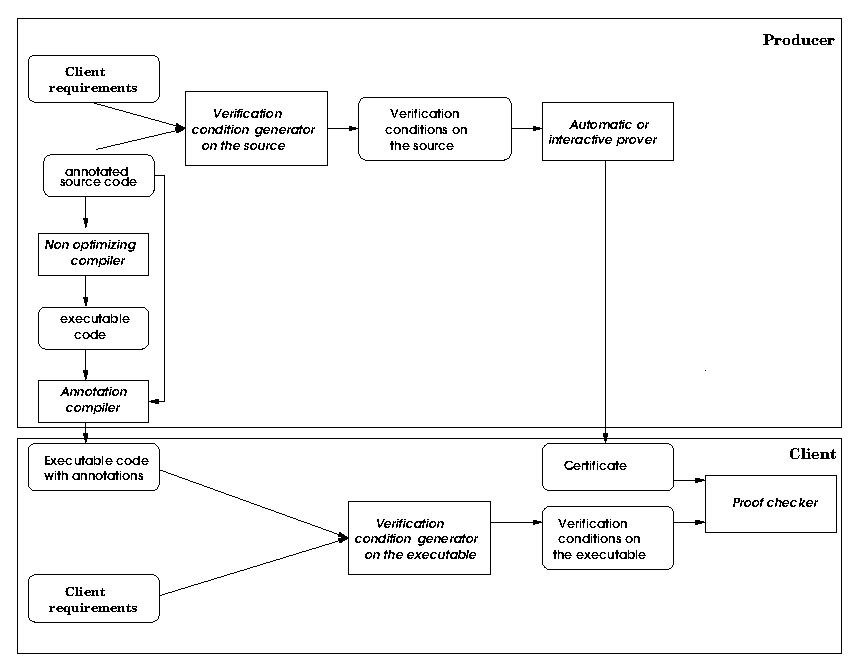
\epsfig{file=figs/PPO.eps}
\caption{\sc Proof preserving compilation for mobile code}
\label{intro:PPO}
\end{center}
%\end{frameit}
\end{figure}


In the following, we present a framework which follows the schemata from Fig. \ref{intro:PPO}  which allows to verify statically bytecode programs 
against potentially non trivial functional and security properties. The framework is tailored to Java bytecode.

  The Java platform  of Sun Microsystems has gained a lot of popularity in industry  for the last two decades.
 The reasons for its  success is that it allows applications to 
 be developed in a high-level language without committing to any
 specific hardware and since it features security mechanisms which
 guarantee the innocuousness of downloaded applications.  
 For instance, smart card applications are relying  on JavaCard, a dialect of Java tailored to small devices.
 Such devices, however, impose  security restrictions  to the software components  they run for which platforms like Java do not provide 
 sufficient mechanisms for their guarantee, e.g. preserving of confidentiality or limited use of computational resources. Moreover,
 the new generation of smart card platforms where installation of  software components after the card has been issued is possible, opens new security problems.
 Another example is the J2ME (which stands for Java 2 Micro Edition) which is widely used in mobile phone software industry.
 Mobile phone users benefit today from the possibility to install new software components on the phone system by the wireless net, 
 however no mechanisms are provided by the Java system to check that they are not malicious.


   \section{Contributions}
   We propose a framework which allows the verification of bytecode programs against complex
   functional and safety properties, which has the following    components.
\begin{description}
     \item [Bytecode Modeling Language] 
         
 %	 Let us see what advocates the need of a
 %	 low level specification language. Traditionally, specification languages were tailored for high level languages.  
 %	 Source  specification allows to express complex functional or security properties about programs.
 %	 Thus, they are successfully  used for software audit and validation. Still, source specification in 
 %	 the context of mobile code does not help a lot for several reasons.

        % As we said above, our objective is to be able  check complex functional or security policies.
 %	 For this, we need a formalism into which properties will be encoded. 

 %	 It is in this perspective, that 
         We define a   specification language for bytecode called BML (short for Bytecode Modeling Language). 
	 BML is the bytecode encoding of an important subset of JML (short for Java Modeling Language). The latter is a rich specification
	 language tailored to Java source programs and allows to specify complex functional properties over Java source programs.
	 Thus, BML inherits the expressiveness of a subset JML and allows to encode potentially 
	 complex functional and security policies over Java bytecode programs.
	 We define an encoding of BML in the class file which is in conformance with the Java Virtual Machine specification \cite{VMSpec}.
	 To our knowledge, BML does not have predecessors that are tailored to Java bytecode.
 
   \item [Verification condition generator for Java bytecode]
         %As we stated above, we target to build a framework where no assumptions for the compiler are made.
	  We propose a verification condition generator (VcGen for short) for Java bytecode which is completely independent from 
	 the source code. The verification condition generator a large subset of Java and deals with
	 arithmetic operations, object creation and manipulation,
	 method invocations, exception throwing and handling, stack manipulation etc.
	 The verification condition relies on a standard weakest predicate transformer function and we
	 have proved its soundness relative to a Java operational semantics.
	 We have an implementation which is integrated in Jack (short for Java Applet Correctness Kit) \cite{BRL-JACK} which is a user friendly 
	 plugin for the eclipse ide \footnote{http://www.eclipse.org/}. 
	 
 

   \item [Compiler from source to bytecode annotations]
         We define a compiler from JML to BML which  
	 allows Java  bytecode benefit from the JML source specification.
	 The compiler does not depend on a particular Java compiler.
	 The JML compilation results in enriching the class file with the BML
	 encoding of the specification.
	 
	 %For properties like well typedness specification can be inferred automatically,
	 %but in the general case and especially in the case of complex properties this problem is not decidable.  
	 %Thus, for more sophisticated policies, an automatic inference will not work.
    \item[Equivalence between source and bytecode proof obligations] Such an equivalence is useful when programs and requirements over them are complex.
         In this case, an interactive verification procedure over the source code  could be helpful.
	 (e.g. proving the verification conditions in an interactive theorem prover).
	 First, interactive  procedure is suitable where automatic decision procedures will not cope with
	 difficult theorems which is potentially the case for sophisticated security policies or functional requirements. 
	 Second, using verification on source code is useful as program bugs and errors can be easily identified and corrected.
	 Because of the relative equivalence between source and bytecode proof obligations, 
	 once the verification conditions over the source and the program requirements expressed as specifications are
	 proved the bytecode and the certificate (the proof of the verification conditions) produced over the source
	 can be shipped  to the client.


\end{description}


We have applied our verification condition generator in two cases. The first one is the verification of constraint memory consumption policies.
 Indeed, it is an important issue for devices with limited resources as smart cards to have a guarantee that a newly installed application 
will not corrupt the whole system because of malevolent resource usage. In such critical situations, bytecode verification is suitable
as it does not compromise the compiler. This work was published in \cite{gmg05:sefm}.


We have also shown how bytecode verification can be applied to  bytecode to native compiler optimizations. Because the verification is performed
on bytecode, we can relate verification conditions to the particular program point to which they refer. This helps to identify
the program points which can be optimized. This gave issue to the publication \cite{DBLP:conf/cardis/CourbotPGV06}. 
	 

% A natural continuation of the present ideas is putting together the bytecode verification condition generator, 
%	 the  BML language and the equivalence between source and bytecode verification conditions into a Proof Carrying Code framework for complex policies.
%	 In such a framework, the client
%	 will, as usual, rely  on the bytecode verification condition generator and  the certificate sent by the client. 
%	 However, differently from the existing schemes for PCC, the producer site will generate \textit{interactively} the certificate (formal proof) 
%	 over the \textit{source code}. This is motivated by the fact that the client policies may be non trivial and making an interactive proof over the source
%	 code will make finding the proof realistic.
\section{Related techniques}

There exists different techniques for establishing that a program respects certain condition. Here, we make a brief review:

\begin{description}
  
  

   % bytecode verification
   \item [type based verification techniques] 
     This approach does not need the presence of the source code neither require to trust the compiler as
     the checks can be done directly on bytecode. In particular, a typical example is the Java bytecode
     verifier (see \cite{Ljbc}) which is part of the JVM. The bytecode verifier performs static analysis over the bytecode yet,
     it can only guarantee that  the code is well typed and well structured or in other words that the
     bytecode does not corrupt the performance of the virtual machine. 

   % dynamic checks  
   \item [dynamic checks] This approach consists in performing checks dynamically on execution time.    
     However, the performance is compromised especially in the case of 
     devices with limited resources.  For example,
     the Java security architecture ensures that applications will not
     perform illegal memory accesses through stack inspection, which
     performs access control during execution
   
   %PCC
   %  \item[proof carrying code]
    %   The Proof Carrying Code paradigm (PCC) and the certifying compiler \cite{DesNecLee98} are another alternative.
     %  In this architecture, untrusted code
     %  %  is accompanied by a proof for its safety w.r.t. to some safety property and the code receiver has  to generate the 
     %  verification conditions and type check the proof against them. 
     %  The proof is generated automatically by the certifying compiler for properties like well typedness or safe memory access. 
     %  As the certifying compiler is designed to be completely automatic, it will not be able to deal with rich functional or security properties. 
     


\end{description}





\section{Plan of the thesis}


The present thesis is organized as follows. In the next Chapter \ref{javaVerif}, we give an overview of
the basic ideas in Java source verification. We present there the JML language, a Java like source language and verification condition generator
for the source language. We also discuss different approaches in program verification using program logic.
Chapter \ref{opSem:prelim} presents
 the bytecode language and its operational semantics which will be used all along the thesis for the definition of the verification condition generator and the proof
of its soundness. 
Chapter \ref{bcsl} presents the syntax and semantics of the Bytecode Modeling Language (BML) and the compiler from JML to BML. 
Chapter \ref{assertLang} presents the assertion language and its formal semantics which the verification calculus manipulates. 
In Chapter \ref{wpGeneral}, we turn to the definition of the verification condition generator and Chapter \ref{proofGeneral}
 presents the proof of its soundness. In Chapter \ref{pogEquiv}, we shall focus on the relation between 
verification conditions on source and bytecode level and we shall see under what conditions they are the same modulo names and basic types. 
Chapter \ref{applications:memory} presents an application of the bytecode verification condition generator and BML to the verification of constraint memory consumption
policies. Chapter \ref{applications:optimComp} shows how we can build a Java-to-Native compiler using our verification framework.




